% arara: lualatex: {shell: 1}
\documentclass{article}
\newif\ifprompts{}
\promptstrue{}
% \usepackage{fontspec}
\usepackage[rgb,dvipsnames]{xcolor}
\usepackage[T1]{fontenc}
\usepackage{mathpazo}
\usepackage[letterpaper,margin=1.5in]{geometry}
\usepackage[inline]{enumitem}
%\usepackage{makecell}
%\usepackage{tabu}
\usepackage{multirow}
%\usepackage{multicol}
\usepackage{paracol}
%\usepackage{arydshln}
%\usepackage{subcaption}
\usepackage{booktabs}
\usepackage{array}   % for \newcolumntype macro
\usepackage{hyperref}
\usepackage[backend=biber,style=alphabetic,sorting=ynt]{biblatex}
%\usepackage{float}
%\usepackage{endfloat}
%\usepackage[nomarkers,figuresonly]{endfloat}
%\usepackage[nofiglist,nomarkers]{endfloat}
\usepackage{adjustbox}
\usepackage{caption}
%\usepackage[export]{adjustbox}[2011/08/13]
%\usepackage{graphicx}
\usepackage{amsmath}
\usepackage{amssymb}
\usepackage{amsthm}
\usepackage{mathrsfs}
\usepackage{mathtools}
\usepackage{thmtools}
%\usepackage{calc}
\usepackage{xfrac}
\usepackage[nameinlink]{cleveref}
\usepackage{tikz}
\usetikzlibrary{calc,patterns,decorations.markings,arrows.meta}
\usepackage{pgfplots}
%\usepackage{nth}
\usepackage{cancel}
%\usepackage{comment}
\usepackage{clrscode}
\usepackage{fancyvrb}
\usepackage{minted}

% Minted/code block setup
\setmonofont[Scale=MatchLowercase,Contextuals={Alternate}]{FuraCode Nerd Font}
%\setminted{frame=lines,framesep=1em,fontsize=\small}
\usemintedstyle{gruvbox-light}
\setminted{autogobble,breaklines}

% My colors
\definecolor{colorA}{HTML}{BF4040}
\definecolor{colorB}{HTML}{BF8040}
\definecolor{colorC}{HTML}{4080BF}
\definecolor{colorD}{HTML}{40BFBF}

% Hyperref setup
\hypersetup{
    colorlinks=true,
    linkcolor=colorC,
    urlcolor=colorB,
    citecolor=colorA,
}

%\newcolumntype{C}{>{\begin{math}}c<{\end{math}}}
%\DeclareMathOperator{\SPN}{\text{SPN}}

% Colored left-bar
\newlength{\leftbarwidth}
\setlength{\leftbarwidth}{3pt}
\newlength{\leftbarsep}
\setlength{\leftbarsep}{10pt}
\newcommand*{\leftbarcolorcmd}{\color{leftbarcolor}}
\colorlet{leftbarcolor}{black}
\renewenvironment{leftbar}[1][black]{%
    \colorlet{leftbarcolor}{#1}
    \def\FrameCommand{{\leftbarcolorcmd{\vrule width \leftbarwidth\relax\hspace {\leftbarsep}}}}%
    \MakeFramed {\advance \hsize -\width \FrameRestore }%
}{%
    \endMakeFramed
}

% Theorem environments
\theoremstyle{plain}
\newtheorem{THM}{Theorem}
\newtheorem*{THM*}{Theorem}
\newtheorem{lemma}{Lemma}
\newtheorem*{lemma*}{Lemma}
\newtheorem*{claim}{Claim}
\newtheorem*{cor}{Corollary}
\newtheorem{prop*}{Proposition}
\newtheorem*{conj}{Conjecture}
\theoremstyle{remark}
\newtheorem*{example*}{Example}
\theoremstyle{definition}
\newtheorem*{definition*}{Definition}
\newenvironment{thm}%
  {\begin{leftbar}[colorA]\begin{THM}
}{%
  \end{THM}\end{leftbar}
}
\newenvironment{thm*}%
  {\begin{leftbar}[colorA]\begin{THM*}
}{%
  \end{THM*}\end{leftbar}
}
\newenvironment{prop}%
  {\begin{leftbar}[colorB]\begin{prop*}
}{%
  \end{prop*}\end{leftbar}
}
\newenvironment{definition}%
  {\begin{leftbar}[colorC]\begin{definition*}
}{%
  \end{definition*}\end{leftbar}
}
\newenvironment{example}%
  {\begin{leftbar}[colorD]\begin{example*}
}{%
  \end{example*}\end{leftbar}
}

% Math functions
\newcommand{\spm}[1]{\left(\begin{smallmatrix}#1\end{smallmatrix}\right)}
\newcommand{\gen}[1]{{\langle{#1}\rangle}}
\newcommand{\angvec}[1]{\gen{#1}}
\newcommand{\oldvec}[1]{\vec{#1}}
\renewcommand{\vec}[1]{\boldsymbol{#1}}

% Math operators and symbols
\DeclareMathOperator{\ZZ}{\mathbb{Z}}
\DeclareMathOperator{\QQ}{\mathbb{Q}}
\DeclareMathOperator{\NN}{\mathbb{N}}
\DeclareMathOperator{\RR}{\mathbb{R}}
\DeclareMathOperator{\CC}{\mathbb{C}}
\DeclareMathOperator{\FF}{\mathbb{F}}
\DeclareMathOperator{\calA}{{\mathcal{A}}}
\DeclareMathOperator{\calB}{{\mathcal{B}}}
\DeclareMathOperator{\calC}{{\mathcal{C}}}
\DeclareMathOperator{\calD}{{\mathcal{D}}}
\DeclareMathOperator{\calE}{{\mathcal{E}}}
\DeclareMathOperator{\calF}{{\mathcal{F}}}
\DeclareMathOperator{\calG}{{\mathcal{G}}}
\DeclareMathOperator{\calH}{{\mathcal{H}}}
\DeclareMathOperator{\calI}{{\mathcal{I}}}
\DeclareMathOperator{\calJ}{{\mathcal{J}}}
\DeclareMathOperator{\calK}{{\mathcal{K}}}
\DeclareMathOperator{\calL}{{\mathcal{L}}}
\DeclareMathOperator{\calN}{{\mathcal{N}}}
\DeclareMathOperator{\calP}{{\mathcal{P}}}
\DeclareMathSymbol{\sminus}{\mathbin}{AMSa}{"39}
\DeclareMathOperator{\tr}{tr}
\DeclareMathOperator{\lcm}{lcm}
%\DeclareMathOperator{\Pr}{\mathrm{\textbf{Pr}}}

% Paired math operators
\DeclarePairedDelimiter{\abs}{\lvert}{\rvert}
\DeclarePairedDelimiter{\ceil}{\lceil}{\rceil}
\DeclarePairedDelimiter{\floor}{\lfloor}{\rfloor}

% Math helper functions
\newcommand{\norm}[1]{\lVert{}#1\rVert{}}
\newcommand{\mx}[1]{\begin{matrix}#1\end{matrix}}
\newcommand{\bmx}[1]{\begin{bmatrix}#1\end{bmatrix}}
\newcommand{\pmx}[1]{\begin{pmatrix}#1\end{pmatrix}}
\newcommand{\sbmx}[1]{{\left[\begin{smallmatrix}#1\end{smallmatrix}\right]}}
\newcommand{\spmx}[1]{{\left(\begin{smallmatrix}#1\end{smallmatrix}\right)}}
\newcommand*\circled[3]{%
    \tikz[baseline=(char.base)]{
        \node[circle,draw=#1,inner sep=#2] (char) {#3};
    }
}

% Prompt
%\newif\ifprompts{}
\ifprompts
    \newenvironment{prompt}{\begin{em}\textbf{Prompt:}}{\end{em}}
    %\newenvironment{prompt}{\begin{em}}{\end{em}}
\else
    \excludecomment{prompt}
\fi
\newcommand\pmt[1]{\begin{prompt}#1\end{prompt}}

\pgfplotsset{compat=1.17}

% Style
%\renewcommand\labelitemi{\small$\bullet$}
%\setmonofont[Scale=MatchLowercase,Contextuals={Alternate}]{FuraCode Nerd Font}
%\setminted{frame=lines,framesep=1em,fontsize=\small}
\setlength\parindent{0em}
\setlength\parskip{1em}
%\usemintedstyle{solarizedlight}
%\renewcommand\theadalign{bc}
%\renewcommand\theadfont{\bfseries}
%\renewcommand\theadgape{\Gape[4pt]}
%\renewcommand\cellgape{\Gape[4pt]}
\newcommand\Item{\item\mbox{}}

\makeatletter
\renewenvironment{cases}[1][l]{\matrix@check\cases\env@cases{#1}}{\endarray\right.}
\def\env@cases#1{%
  \let\@ifnextchar\new@ifnextchar
  \left\lbrace\def\arraystretch{1.2}%
  \array{@{}#1@{\quad}l@{}}}
\makeatother

\usepackage{fontspec}
\usepackage[rgb,dvipsnames]{xcolor}
\usepackage[T1]{fontenc}
\usepackage{mathpazo}
\usepackage[letterpaper,margin=1.5in]{geometry}
\usepackage[inline]{enumitem}
%\usepackage{makecell}
%\usepackage{tabu}
\usepackage{multirow}
%\usepackage{multicol}
\usepackage{paracol}
%\usepackage{arydshln}
%\usepackage{subcaption}
\usepackage{booktabs}
\usepackage{array}   % for \newcolumntype macro
\usepackage{hyperref}
\usepackage[backend=biber,style=alphabetic,sorting=ynt]{biblatex}
%\usepackage{float}
%\usepackage{endfloat}
%\usepackage[nomarkers,figuresonly]{endfloat}
%\usepackage[nofiglist,nomarkers]{endfloat}
\usepackage{adjustbox}
\usepackage{caption}
%\usepackage[export]{adjustbox}[2011/08/13]
%\usepackage{graphicx}
\usepackage{amsmath}
\usepackage{amssymb}
\usepackage{amsthm}
\usepackage{mathrsfs}
\usepackage{mathtools}
\usepackage{thmtools}
%\usepackage{calc}
\usepackage{xfrac}
\usepackage[nameinlink]{cleveref}
\usepackage{tikz}
\usetikzlibrary{calc,patterns,decorations.markings,arrows.meta}
\usepackage{pgfplots}
%\usepackage{nth}
\usepackage{cancel}
%\usepackage{comment}
\usepackage{clrscode}
\usepackage{fancyvrb}
\usepackage{minted}

% Minted/code block setup
\setmonofont[Scale=MatchLowercase,Contextuals={Alternate}]{FuraCode Nerd Font}
%\setminted{frame=lines,framesep=1em,fontsize=\small}
\usemintedstyle{gruvbox-light}
\setminted{autogobble,breaklines}

% My colors
\definecolor{colorA}{HTML}{BF4040}
\definecolor{colorB}{HTML}{BF8040}
\definecolor{colorC}{HTML}{4080BF}
\definecolor{colorD}{HTML}{40BFBF}

% Hyperref setup
\hypersetup{
    colorlinks=true,
    linkcolor=colorC,
    urlcolor=colorB,
    citecolor=colorA,
}

%\newcolumntype{C}{>{\begin{math}}c<{\end{math}}}
%\DeclareMathOperator{\SPN}{\text{SPN}}

% Colored left-bar
\newlength{\leftbarwidth}
\setlength{\leftbarwidth}{3pt}
\newlength{\leftbarsep}
\setlength{\leftbarsep}{10pt}
\newcommand*{\leftbarcolorcmd}{\color{leftbarcolor}}
\colorlet{leftbarcolor}{black}
\renewenvironment{leftbar}[1][black]{%
    \colorlet{leftbarcolor}{#1}
    \def\FrameCommand{{\leftbarcolorcmd{\vrule width \leftbarwidth\relax\hspace {\leftbarsep}}}}%
    \MakeFramed {\advance \hsize -\width \FrameRestore }%
}{%
    \endMakeFramed
}

% Theorem environments
\theoremstyle{plain}
\newtheorem{THM}{Theorem}
\newtheorem*{THM*}{Theorem}
\newtheorem{lemma}{Lemma}
\newtheorem*{lemma*}{Lemma}
\newtheorem*{claim}{Claim}
\newtheorem*{cor}{Corollary}
\newtheorem{prop*}{Proposition}
\newtheorem*{conj}{Conjecture}
\theoremstyle{remark}
\newtheorem*{example*}{Example}
\theoremstyle{definition}
\newtheorem*{definition*}{Definition}
\newenvironment{thm}%
  {\begin{leftbar}[colorA]\begin{THM}
}{%
  \end{THM}\end{leftbar}
}
\newenvironment{thm*}%
  {\begin{leftbar}[colorA]\begin{THM*}
}{%
  \end{THM*}\end{leftbar}
}
\newenvironment{prop}%
  {\begin{leftbar}[colorB]\begin{prop*}
}{%
  \end{prop*}\end{leftbar}
}
\newenvironment{definition}%
  {\begin{leftbar}[colorC]\begin{definition*}
}{%
  \end{definition*}\end{leftbar}
}
\newenvironment{example}%
  {\begin{leftbar}[colorD]\begin{example*}
}{%
  \end{example*}\end{leftbar}
}

% Math functions
\newcommand{\spm}[1]{\left(\begin{smallmatrix}#1\end{smallmatrix}\right)}
\newcommand{\gen}[1]{{\langle{#1}\rangle}}
\newcommand{\angvec}[1]{\gen{#1}}
\newcommand{\oldvec}[1]{\vec{#1}}
\renewcommand{\vec}[1]{\boldsymbol{#1}}

% Math operators and symbols
\DeclareMathOperator{\ZZ}{\mathbb{Z}}
\DeclareMathOperator{\QQ}{\mathbb{Q}}
\DeclareMathOperator{\NN}{\mathbb{N}}
\DeclareMathOperator{\RR}{\mathbb{R}}
\DeclareMathOperator{\CC}{\mathbb{C}}
\DeclareMathOperator{\FF}{\mathbb{F}}
\DeclareMathOperator{\calA}{{\mathcal{A}}}
\DeclareMathOperator{\calB}{{\mathcal{B}}}
\DeclareMathOperator{\calC}{{\mathcal{C}}}
\DeclareMathOperator{\calD}{{\mathcal{D}}}
\DeclareMathOperator{\calE}{{\mathcal{E}}}
\DeclareMathOperator{\calF}{{\mathcal{F}}}
\DeclareMathOperator{\calG}{{\mathcal{G}}}
\DeclareMathOperator{\calH}{{\mathcal{H}}}
\DeclareMathOperator{\calI}{{\mathcal{I}}}
\DeclareMathOperator{\calJ}{{\mathcal{J}}}
\DeclareMathOperator{\calK}{{\mathcal{K}}}
\DeclareMathOperator{\calL}{{\mathcal{L}}}
\DeclareMathOperator{\calN}{{\mathcal{N}}}
\DeclareMathOperator{\calP}{{\mathcal{P}}}
\DeclareMathSymbol{\sminus}{\mathbin}{AMSa}{"39}
\DeclareMathOperator{\tr}{tr}
\DeclareMathOperator{\lcm}{lcm}
%\DeclareMathOperator{\Pr}{\mathrm{\textbf{Pr}}}

% Paired math operators
\DeclarePairedDelimiter{\abs}{\lvert}{\rvert}
\DeclarePairedDelimiter{\ceil}{\lceil}{\rceil}
\DeclarePairedDelimiter{\floor}{\lfloor}{\rfloor}

% Math helper functions
\newcommand{\norm}[1]{\lVert{}#1\rVert{}}
\newcommand{\mx}[1]{\begin{matrix}#1\end{matrix}}
\newcommand{\bmx}[1]{\begin{bmatrix}#1\end{bmatrix}}
\newcommand{\pmx}[1]{\begin{pmatrix}#1\end{pmatrix}}
\newcommand{\sbmx}[1]{{\left[\begin{smallmatrix}#1\end{smallmatrix}\right]}}
\newcommand{\spmx}[1]{{\left(\begin{smallmatrix}#1\end{smallmatrix}\right)}}
\newcommand*\circled[3]{%
    \tikz[baseline=(char.base)]{
        \node[circle,draw=#1,inner sep=#2] (char) {#3};
    }
}

% Prompt
%\newif\ifprompts{}
\ifprompts
    \newenvironment{prompt}{\begin{em}\textbf{Prompt:}}{\end{em}}
    %\newenvironment{prompt}{\begin{em}}{\end{em}}
\else
    \excludecomment{prompt}
\fi
\newcommand\pmt[1]{\begin{prompt}#1\end{prompt}}

\pgfplotsset{compat=1.17}

% Style
%\renewcommand\labelitemi{\small$\bullet$}
%\setmonofont[Scale=MatchLowercase,Contextuals={Alternate}]{FuraCode Nerd Font}
%\setminted{frame=lines,framesep=1em,fontsize=\small}
\setlength\parindent{0em}
\setlength\parskip{1em}
%\usemintedstyle{solarizedlight}
%\renewcommand\theadalign{bc}
%\renewcommand\theadfont{\bfseries}
%\renewcommand\theadgape{\Gape[4pt]}
%\renewcommand\cellgape{\Gape[4pt]}
\newcommand\Item{\item\mbox{}}

\makeatletter
\renewenvironment{cases}[1][l]{\matrix@check\cases\env@cases{#1}}{\endarray\right.}
\def\env@cases#1{%
  \let\@ifnextchar\new@ifnextchar
  \left\lbrace\def\arraystretch{1.2}%
  \array{@{}#1@{\quad}l@{}}}
\makeatother

\setlist{
   itemsep=0em,
   %first={\setlength{\parskip}{1em}}
}
\setlength{\parindent}{0em}
\setlength{\parskip}{0.5em}
% \newenvironment{code}{\captionsetup{type=listing}}{}
% \newcommand{\colorA}{RoyalBlue}
% \newcommand{\colorB}{PineGreen}
% \newcommand{\colorC}{OrangeRed}
% \addbibresource{references.bib}

\newcommand{\moles}{\mathrm{mol}}
% \newcommand{\joules}{\mathrm{mol}}
\newcommand{\Hyd}{\mathrm{H}_2}
\newcommand{\Nit}{\mathrm{N}_2}
\newcommand{\Ox}{\mathrm{O}_2}
\newcommand{\Pol}{\mathrm{X}}
\newcommand{\CDiox}{\mathrm{CO}_2}
\newcommand{\Water}{\mathrm{H}_2\mathrm{O}}
\newcommand{\NiOx}{\mathrm{N}_2\mathrm{O}}

\newcommand\pgfmathparseFPU[1]{
    \begingroup%
        \pgfkeys{/pgf/fpu,/pgf/fpu/output format=fixed}
        \pgfmathparse{#1}
        \pgfmathsmuggle\pgfmathresult
    \endgroup
}
% \def\GasConstant{8.314}
% \def\vF{1000}
% \def\tC{230}
% \def\tH{2300}
\def\SAMPLES{7}
\newcommand{\setupparams}[6]{%
    \pgfmathsetmacro{\GasConstant}{8.314}
    \pgfmathsetmacro{\vF}{1000}
    \pgfmathsetmacro{\pF}{#1}
    \pgfmathsetmacro{\tF}{#2}
    \pgfmathparseFPU{\pF/\tF*\vF/\GasConstant)}\pgfmathsetmacro{\nF}{\pgfmathresult}
    \pgfmathsetmacro{\pT}{#3}
    \pgfmathsetmacro{\tT}{#4}
    \pgfmathparseFPU{\pT/\tT*\vF/\GasConstant)}\pgfmathsetmacro{\nT}{\pgfmathresult}
    \pgfmathsetmacro{\tC}{#5}
    \pgfmathsetmacro{\tH}{#6}
    \pgfmathsetmacro{\rG}{0}
    \pgfmathparseFPU{\nF-(\nT*(\tT-\tH))/(\tF-\tH)}\pgfmathsetmacro{\rR}{\pgfmathresult}
    \pgfmathparseFPU{\nF-(\nT*(\tT-\tC))/(\tF-\tC)}\pgfmathsetmacro{\rB}{\pgfmathresult}
}
\newcommand{\surf}{%
    \addplot3[%
        surf,
        samples=\SAMPLES,
        samples y=\SAMPLES,
        opacity=0.5,
        domain=0:\nF,
        domain y=\tC:\tH,
        variable=\nR,
    ]
    {(\tT*\nT-\tF*(\nF-\nR))/y};
}
\newcommand{\curve}{%
    \addplot3[%
        thick,
        color=red,
        samples=\SAMPLES,
        samples y=0,
        domain={max(\rG, max(\rR, \rB))}:\nF,
        domain y=\tC:\tH,
        variable=\nR,
    ]
    ({\nR},{(\tT*\nT-\tF*(\nF-\nR))/(\nT-\nF+\nR)},{\nT-\nF+\nR});
}
\newcommand{\Surf}[7][1.0]{%
    \setupparams{#2}{#3}{#4}{#5}{#6}{#7}
    \begin{tikzpicture}[scale=#1]
        \begin{axis}[
                title={$P_F=\pF$, $T_F=\tF$, $P_T=\pT$, $T_T=\tT$},
                xlabel=$n_R$, ylabel=$T_I$, zlabel=$n_I$,
                view={-135}{45},
                ymin=\tC, ymax=\tH,
                zmin=0,
            ]
            \surf%
        \end{axis}
    \end{tikzpicture}
}
\newcommand{\Curve}[7][1.0]{%
    \setupparams{#2}{#3}{#4}{#5}{#6}{#7}
    \begin{tikzpicture}[scale=#1]
        \begin{axis}[
                title={$P_F=\pF$, $T_F=\tF$, $P_T=\pT$, $T_T=\tT$},
                xlabel=$n_R$, ylabel=$T_I$, zlabel=$n_I$,
                view={-135}{45},
                ymin=\tC,ymax=\tH,
                zmin=0,
            ]
            \surf%
            \curve%
        \end{axis}
    \end{tikzpicture}
}
\newcommand{\Full}[7][1.0]{%
    \setupparams{#2}{#3}{#4}{#5}{#6}{#7}
    \begin{tikzpicture}[scale=#1]
        \begin{axis}[
                title={$P_F=\pF$, $T_F=\tF$, $P_T=\pT$, $T_T=\tT$},
                xlabel=$n_R$, ylabel=$T_I$, zlabel=$n_I$,
                view={-135}{45},
                ymin=\tC, ymax=\tH,
                zmin=0,
            ]
            \surf%
            \curve%
            \filldraw[green]
            (
                {\rG},
                {(\tT*\nT-\tF*\nF)/(\nT-\nF)},
                {\nT-\nF}
            ) circle (2pt) node {};
            \filldraw[red]
            (
                {\rR},
                {\tH},
                {\nT-(\nT*(\tT-\tH))/(\tF-\tH)}
            ) circle (2pt) node {};
            \filldraw[blue]
            (
                {\rB},
                {\tC},
                {\nT-(\nT*(\tT-\tC))/(\tF-\tC)}
            ) circle (2pt) node {};
        \end{axis}
    \end{tikzpicture}
}

\begin{document}

\tableofcontents

\section*{Todo}
\begin{itemize}
    \item Add motivations for calculation specif heat capacities and energies.
        That is, what do these quantities mean?
\end{itemize}

\section{Introduction and Summary}
In this section, I'll first attempt to introduce all relevant mathematical notation;
units, fundamental concepts and gas laws in physics;
and then attempt summarize my solutions to the proposed problem:
\begin{quote}
    \begin{itshape}
        Given a furnace $F$ containing only $\CDiox$ at some arbitrary initial conditions, a source
        $C$ of relatively cold $\CDiox$ and a source $H$ of relatively hot $\CDiox$: is there not
        only some way of constructing a mixture of $H$ and $C$ such that inserting it into $F$
        yields exactly some target temperature $T_T$ and pressure $P_T$ in $F$, but a way in which
        \begin{enumerate*}[label=(\alph*)]
            \item we minimize the amount $n_R$ which is removed from the initial amount of gas, and
            \item we minimize the amounts $n_C$ from $C$ and $n_H$ from $H$ that we are adding?
        \end{enumerate*}
    \end{itshape}
\end{quote}

\subsection{Notation, basic physics, and thermodynamics}

Firstly, I'll often write a closed mixture/volume of gasses as a single capital letter, like $F$ for
furnace, and where I can now use $F$ to symbolically refer to any of the conditions of the furnace.
Formally:
\begin{definition}[$M$ a gas mixture]
    Let $M$ be a mixture/volume/composition of gasses; we write:
    \begin{itemize}
        \item $V_M$ for the total volume in liters of the system in which the mixture is contained,
        \item $n_M$ for the total number of moles in the mixture,
        \item $T_M$ for the temperature of the mixture,
        \item $P_M$ for the total pressure of the mixture,
        \item $C_M$ for the specific heat (capacity) of the mixture, and
        \item $Q_M$ for the total energy of the mixture.
    \end{itemize}
\end{definition}
\begin{note*}
    I use \emph{volume}, \emph{mixture} and \emph{composition} somewhat interchangeably when talking
    about some specific closed amount of gas, and that ``volume'' here has nothing to do with the
    actual volume in liters of the container in which the closed amount of gas sits.

    For example, ``a volume $M$ of gas'' versus ``the volume (in liters) of the
    mixture/composition/volume $M$.''
\end{note*}
\begin{note*}
    Seeing as we're going to be working with equations involving quantities of various units, it's
    going to be important to understand what a particular unit of measurement means and how these
    units relate to one-another. But to understand units is also to have some basic understanding
    of physics and thermodynamics.
    (It's also imperative to understand unit prefixes; like \emph{kilo} $k$ for ``a thousand of'',
    \emph{mega} $M$ for ``a million of'', or \emph{milli} $m$ for ``a millionth of''.)

    Here's sort of a summary introduction to all of these things:
\end{note*}
\begin{definition*}[Moles, volume, temperature, pressure]
    A \emph{mole} (mol) is the base unit of an amount of a substance. A mole of a substance
    contains a particular number of particles of the substance, just as gram of a substance
    contains a certain number of particles, and so the relationship between moles and mass is
    some constant scaling factor (that is, if I have a sample of a substance that is $a$ moles
    and $b$ grams, then there is some number $c$ such that $a=cb$ or $\sfrac{a}{c}=b$ where $c$
    is the scaling factor).

    \emph{Volume} is the quantity of an enclosed space. Where a $m$ meter is the base unit of
    distance, a $L$ liter is the base unit of volume. A single liter is defined as equivalent to
    three cubic meters ($1\cdot\text{L}=1\cdot\text{m}^3$). Particles of gasses are special in
    that they prefer to be evenly spaced apart from one-another while inside some volume. Take
    some amount of gas (some number of moles of gas perhaps) and put it in a volume: a larger
    volume means more space between particles, while a smaller volume means less space between
    particles.

    \emph{Temperature} is the quantity measured in $K$ kelvin that expresses hot or cold, where
    hot and cold are manifestations of the transfer of thermal energy between particles (of
    which all contain some amount of thermal energy). That is, an object is hot relative to its
    colder surroundings if it has more thermal energy that its surroundings, and as a result can
    impart some of its thermal energy to its surroundings: hot things impart energy and become
    colder, cold things absorb energy and become hotter. Considering an amount of gas within a
    volume, though the particles of gas are spaced apart from one-another they are not
    stationary: they move or vibrate relative to their temperature. These movements may cause
    the particles to collide with one-another and with the walls of the container.

    \emph{Pressure} is the quantity that expresses the average amount of force that is being
    exerted upon the area of a surface. A force (measured in newtons) is an influence that can
    causes matter to change velocity (i.e. to push), the actual act of imparting force is called
    work (measured in joules), and the capacity for something to do work is called energy (also
    measured in joules). As mentioned for gas particles in a container, collisions occur between
    the particles and the walls of the container. However much these particles end up on average
    colliding with, or pushing against, the walls of the container is the pressure of the gas
    within the volume, measured as pascals ($\text{Pa}$). A single pascal is defined to be a
    single joule per cubic meter ($\text{J}/\text{m}^3$, or equivalently $\text{J}/\text{L}$
    since $1\cdot\text{L}=1\cdot\text{m}^3$).
\end{definition*}
\begin{definition*}[Specific heat, total energy]
    Informally, the specific heat (capacity) of a substance is the amount of heat/energy (in joules)
    required to increase its temperature by a single degree, and is quantified as joules per mole
    kelvin ($\sfrac{\text{J}}{\text{mol K}}$). Particular substances each have their
    own specific heat (\cref{fig:gas-table}). These quantities are important in that they relate
    energy to substance amount and temperature. Given an amount and temperature of a substance we
    can calculate the energy; given the energy and amount of a substance we can calculate the
    temperature; and given the energy and temperature of a substance we can calculate the amount.

    The total energy then for some amount of a particular kind of gas is simply the specific heat
    multiplied by the amount and the temperature. For example, one-thousand moles of $\CDiox$ at
    273.15 kelvin has a total energy of $1000\cdot 273.15\cdot 27.2=742\text{kJ}$.
\end{definition*}
Secondly, there are seven types of gasses in the game, each with a formula. I use the formulas as
\emph{indices} for the gasses. That is, if I say \emph{the gas $g$}, then what I mean is \emph{the
gas indexed by $g$, an element of the set of gas indices}. I can then use this index $g$ to refer to
the conditions, within a mixture of gasses, of just this one gas indexed by $g$.
\begin{definition}[$g$ a gas index]
    Define the set of gas indices for Stationeers:
    \[
        \calG = \{\Hyd,\Nit,\Ox,\Pol,\CDiox,\Water,\NiOx\}.
    \]
    We assume that the order of these indices is always the same;
    that is, the first element of $\calG$ is always $\Hyd$, the second is always $\Nit$, and so on.

    Let $M$ be a mixture of the gasses indexed by the elements of $\calG$, and
    let $g\in\calG$ (read, $g$ is an element of $\calG\Leftrightarrow g=\Hyd$, or $\Nit$,\ \ldots, or $\NiOx$).
    Then we write:
    \begin{itemize}
        \item $n_M(g)$ for the moles of $g$ (the gas indexed by $g$) within mixture $M$,
        \item $P_M(g)$ for the partial pressure of $g$ within mixture $M$, and
        \item $C_g$ the \href{https://en.wikipedia.org/wiki/Specific_heat_capacity}{specific heat
            (capacity)} of a gas $g$.
    \end{itemize}
    And note that we don't write $T_M(g)$ for the temperature of $g$ in $M$, because every
    particular gas in mixture $M$ has the same temperature. Though, this often \emph{not} true for
    the pressures of each individual constituent gas of a mixture (see Dalton's law,
    \cref{def:daltons}).
\end{definition}
See see \cref{fig:gas-table} for a table of the gasses in Stationeers, their $g$
formulas/indices, and their $C_g$ specific heats.
\begin{note*}[Sets in math]
    A \emph{set} in math is simply a collection of things that are distinct but of the same type,
    are notated with their elements or their definition surrounded by braces, \{ and \}, and are
    often represented by a widely accepted single character or symbol. I say \emph{or} for how they
    are notated because we can define sets in various but equivalent ways: \emph{semantically}, as a
    \emph{finite} or \emph{infinite roster}, or using what's called \emph{set-builder notation}.

    To give examples of these different ways of construction, consider that numbers in general
    are members of sets of other numbers, and often are members of various sets. And often sets
    are \emph{subsets} of other sets; smaller and more restrictive than the outer set. Take first
    for example the \emph{set of integers}, often represented by the symbol $\ZZ$. See the semantic
    definition of an integer in both the semantic and set-builder definitions below:
    \begin{align*}
        \ZZ
        &= \text{ the set of numbers with no fractional part} \\
        &= \{ \ldots, -2, -1, 0, 1, 2, \ldots \}
        = \{ n : \text{$n$ is a number with no fractional part} \}.
    \end{align*}
    Now consider the set $\WW$ of \emph{whole}, or \emph{counting} numbers:
    \[
        \WW = \{ 1, 2, 3, \ldots \} = \{ n: n\in\ZZ, n>0 \}.
    \]
    The colon ($:$) defines rule(s) for set-builder definition, and the symbol $\in$ means ``element
    tof'': that what's on the left is taken to be an element of the set on the right.
    The set we construct by the above rules is then simply the set of all the positive integers---a
    subset of the integers.

    In either example above the roster definitions are infinite roster definitions; we cannot list
    every integer of these sets because there is an infinite number of them. On the other
    hand, a set $\{1,2,3\}=\{n:n\in Z,0<n<4\}$ is finite in its size/in its roster definition.
\end{note*}
\begin{figure}
    \begin{center}
        \begin{tabular}{*3l}
            \toprule
            Name & Formula ($g$) & Specific heat ($C_g$ in $\sfrac{\text{J}}{\text{mol K}}$) \\
            \midrule
            Hydrogen & $\Hyd$ & 20.4 \\
            Nitrogen & $\Nit$ & 20.6 \\
            Oxygen & $\Ox$ & 21.1 \\
            Pollutant & $\Pol$ & 24.8 \\
            Carbon dioxide & $\CDiox$ & 28.2 \\
            Water & $\Water$ & 72 \\
            Nitrous oxide & $\NiOx$ & 23 \\
            \bottomrule
        \end{tabular}
    \end{center}
    \caption{Table of gasses in Stationeers}
    \label{fig:gas-table}
\end{figure}

All but the last of these conditions can be determined without much calculation; in particular $n_M$
the total moles, $T_M$ temperature and $P_M$ pressure can all be read directly from a furnace/pipe
analyzer/tank in game, and $n_M(g)$ moles of the particular gas $g$ can be calculated simply as the
ratio of the gas times the total moles:
\[
    n_M(g) = \text{(ratio of $g$ in $M$)}\cdot n_M,
    \text{ where } 0 \le \text{ratio of $g$ in $M$} \le 1.
\]
Note that if $M$ consists of only one kind of gas (which I index as $g^*$):
\[
    \text{if } 1 = \text{(ratio of $g^*$ in $M$)}
    \Rightarrow
    n_M(g^*) = 1\cdot n_M = n_M.
\]

\subsection{Gas laws}

Gasses in Stationeers obey some of the ideal gas laws from real life.
First, lets know how to calculate the specific heat of a mixture of gasses.
Recall that a gas, indexed by $g\in\calG$, has a specific heat $C_g$ (\cref{fig:gas-table}).
\begin{definition}[Specific heat capacity of a gas mixture]
    Let $M$ be a mixture of the $\calG$ gasses. The specific heat of the mixture ($C_M$) is given by
    the sum of the products of the molar ratios of the gasses in the mixtures and their respective
    specific heats. We can notate this mathematically in a few ways:
    \[
        C_M
        = \frac{n_M(\Hyd)}{n_M}C_{\Hyd}
        + \frac{n_M(\Nit)}{n_M}C_{\Nit}
        + \cdots
        + \frac{n_M(\NiOx)}{n_M}C_{\NiOx}
        = \sum_{g\in\calG} \frac{n_M(g)}{n_M}C_g
    \]
    Or as the dot-product ($\cdot$) of vectors:
    \begin{equation}
        C_M = (\vec{n}_M \cdot \vec{C}_{\calG})\frac{1}{n_M}
    \end{equation}
    Where $\vec{n}_M$ is the vector of the moles per gas in $M$, and
    where $\vec{C}_{\calG}$ is the vector of the specific heats of each gas:
    \begin{align*}
        \vec{n}_M
        &= \angvec{n_M(\Hyd),n_M(\Nit),\ldots,n_M(\NiOx)}
        = \angvec{n_M(g):g\in\calG} \\
        \vec{C}_{\calG}
        &= \angvec{C_{\Hyd},C_{\Nit},\ldots,C_{\NiOx}}
        = \angvec{C_g:g\in\calG}.
    \end{align*}
\end{definition}
\begin{note*}[If you're unfamiliar with summation notation]

    A sum exactly what you think it is: $a+b$, two things added together.
    If you want to add/sum more than two things you can of course write it out:
    $a + b + c + d$.
    And if there's a lot of things to sum up, and there's some sort of logical
    progression in the sequence of things you're summing as well as a logical end point,
    then you can use ellipses:
    $1 + 2 + 3 + \cdots + 99 + 100$.

    But another, more compact, way to notate this is is \emph{summation notation}.
    Summation notation uses the symbol capital sigma $\sum$ to denote a summation,
    and uses some kind of an \emph{index} to designate where we start in the sum, and
    sometimes where to end.
    For example, the following sum says that we're letting $i$ be our index, that we start with
    $i$ being 1, we stop when $i$ is 100, and after each $i$ we move onto the next $i$
    ($i=1,2,3,\ldots,99,100$). What we're summing are the numbers $x_i$ indexed by $i$:
    \[
        \sum_{i=1}^{100} x_i \quad \text{(for whatever number $x_i$ is)}.
    \]
    In English we would say ``take the sum of the values $x_i$ for each $i$ in the range
    1 to 100 inclusive,'' where \emph{inclusive} means we include $x_{100}$ in the sum, as
    opposed to \emph{exclusive} where we would exclude $x_{100}$. We also might write this range
    of 1 to 100 inclusive as $[1,100]$; versus $[1,100)$ meaning we don't include 100, $(1,100]$
    meaning we don't include 1 but \emph{do} include 100, and $(1,100)$ where we don't include
    either 1 nor 100.

    For a less abstract example, consider the sum of the first 100 positive integers:
    \[
        \sum_{x=1}^{100} x
        = 1 + 2 + 3 + \cdots + 99 + 100.
    \]
    However, the index need not be a number. A common way of expressing indices is via sets, and is
    to say ``take the sum of this expression indexed by every element of the given set.''
    For example: $\sum_{g\in\calG}C_g = $ the sum of the specific heats for each gas indexed by $g$
    in the set of gas indices $\calG$.
\end{note*}
\begin{note*}[If you're unfamiliar with vectors and dot-products]

    Consider a vector to be a list of numbers.
    For example, here are two vectors, $\vec x$ and $\vec y$, of size 3:
    \[
        \vec x = \angvec{x_0,x_1,x_2}, \quad
        \vec y = \angvec{y_0,y_1,y_2}.
    \]
    The dot product ($\cdot$) of $\vec x$ and $\vec y$ (written $\vec x\cdot\vec y$) is given
    as the sum of the products of the corresponding entries of $\vec x$ and $\vec y$:
    \[
        \vec x\cdot\vec y
        = \angvec{x_0,x_1,x_2}\cdot\angvec{y_0,y_1,y_2}
        = x_0 y_0+x_1 y_1+x_2 y_2.
    \]
\end{note*}
Note that if $M$ consists of only one kind of gas $g^*$, then the ratio of $g^*\in\calG$ in $M$ is
one, and the ratio of $g\in\calG\setminus g^*$ in $M$ is zero. And so:
\[
    n_F(g) = \begin{cases}
        n_F(g) = n_F, & \text{if } g = g^* \\
        n_F(g) = 0, & \text{if } g \ne g^* \\
    \end{cases}.
\]
(We read $g\in
\calG\setminus g^*$ as: $g$ is an element of the set $\calG\setminus g^*$, where $\calG\setminus
g^*$ is the set $\calG$ but with the $g^*$ element removed.)
\begin{example*}[Using summation notation]
    Suppose $F$ our furnace contains 10 moles of each kind of gas, of which there are seven.

    Then $n_F=70$, and:
    \begin{align*}
        C_F
        = \sum_{g\in\calG}\frac{n_F(g)}{n_F}C_g
        &= \frac{n_F(\Hyd)}{n_F}C_{\Hyd}+\frac{n_F(\Nit)}{n_F}C_{\Nit}+\cdots+\frac{n_F(\NiOx)}{n_F}C_{\NiOx} \\
        &= \frac{10}{70}\left(20.4 + 20.6 + 21.1 + 24.8 + 28.2 + 72 + 23\right)
        = 30.01
    \end{align*}
\end{example*}
\begin{example*}[Using vector notation]
    Suppose $F$ our furnace contains 70 moles of only $g^*=\CDiox$.

    Then $n_F=n_F(\CDiox)=70$, and:
    \begin{gather*}
        n_F(g) = \begin{cases}
            n_F(g) = n_F, & \text{if } g = \CDiox \\
            n_F(g) = 0, & \text{if } g \ne \CDiox \\
        \end{cases}, \\
        \begin{aligned}
            C_F
            &= \left(\vec{n}_F \cdot \vec{C}_{\calG}\right)\frac{1}{n_F} \\
            &=
            \left(\angvec{0,0,0,0,70,0,0}
            \cdot
            \angvec{C_{\Hyd},C_{\Nit},C_{\Ox},C_{\Pol},C_{\CDiox},C_{\Water},C_{\NiOx}}\right)
            \frac{1}{70}
            \\
            &= (70\cdot C_{\CDiox})\frac{1}{70} = C_{\CDiox}
        \end{aligned}
    \end{gather*}
\end{example*}
This reduction of a volume's specific heat to a constant is one reason why I prefer a single gas
($\CDiox$) design; it reduces many of the later problems from problems of differential equations to
simple problems of algebra. The other reason is that $\CDiox$ is plentiful, both as at atmospheric
gas on planets like Mars and Venus and as a byproduct of combustion.

In terms of gas laws, the model in Stationeers obeys the following laws for a fixed volume of gas.

\begin{definition}[Gay-Lussac's law]
    \begin{equation}
        P_1 T_2=P_2 T_1
        \label{eq:gay-lussac}
    \end{equation}
    Change in pressure is directly proportional to change in temperature.
    \begin{note*}
        In Stationeers this law is \emph{only half-obeyed}!
        Pressure is dependent on temperature (i.e. changing the temperature in a fixed volume
        expectedly affects pressure proportionally), but temperature is \emph{not} dependent on
        temperature (i.e. changing the pressure/removing gas does \emph{not} affect temperature).

        (Also note that we wont actually be using this law for solving the problem, but it is very
        important to understand in general; especially the above caveat.)
    \end{note*}
\end{definition}

\begin{definition}[Ideal/combined gas law]
    \begin{equation}
        PV=nRT
        \label{eq:ideal}
    \end{equation}
    Where $R=8.314$ (joules per mole kelvin)
    is the \href{https://en.wikipedia.org/wiki/Gas_constant}{universal gas constant}.
\end{definition}

\begin{definition}[Dalton's law of partial pressures]
    \label{def:daltons}
    \begin{equation}
        P
        = P(\Hyd)+P(\Nit)+P(\Ox)+P(\Pol)+P(\CDiox)+P(\Water)+P(\NiOx)
        = \sum_{g\in\calG}P(g)
        \label{eq:partial-p}
    \end{equation}
    The pressure in the volume is the sum of partial pressures of the constituent gasses.
\end{definition}

\begin{definition}[Energy of a volume gas]
    The energy of a volume of gas with temperature $T$, number of moles $n$, and
    (combined) specific heat $C$ is given by $TnC$.
\end{definition}

Furthermore, the game model satisfies these other equations.
Given volumes $A$ and $B$, and $C$ the result of combining $A$ and $B$:
\begin{flalign}
    &n_C = n_A + n_B &
    &\text{(moles are additive)} & \label{eq:n-combine} \\
    &C_C = \left((\vec{n}_A+\vec{n}_B)\cdot\vec{C}_{\calG}\right)\frac{1}{n_C} &
    &\text{(combined specific heat of a single mixture)} & \label{eq:C-combine} \\
    &T_C n_C C_C = T_A n_A C_A+T_B n_B C_B &
    &\text{(combined energies of two mixtures)} & \label{eq:energy-combine}
\end{flalign}
\begin{note*}[Why we need to consider combined energies]
    When we mix a volume of gas $A$ with another $B$ into a combined volume $C$, the resulting
    combined energy is entirely dependent on not only the temperatures of $A$ and $B$, but also
    the compositions of $A$ and $B$. There is a lot more energy in one mole of $\Water$ at $273.15$
    kelvin than there is in one mole of $\CDiox$ (precisely, 72 joules to 28.2 joules).
    When we combine $A$ and $B$ we create a new composition, but the 
\end{note*}
With all this notation and all these gas equations in mind,
we move onto solving the proposed problem.

\pagebreak
\subsection{Solving the problem}

To draft up the scenario:

\emph{(Initial conditions)}
A furnace already contains some amount of ``hot'' $\CDiox$ as a starter. We add the reagents for
some alloy, releasing some other gasses into the furnace mix. We then filter out all gases except
for the $\CDiox$, returning the $\CDiox$ back into the furnace, leaving the furnace with only
$\CDiox$ gas but also the reagents for the alloy. For the alloy we require some specific
temperature, $T_T$ (target temperature), and pressure, $P_T$ (target pressure); we'll consider these
to be the minimum of whatever the alloy ranges are. Lastly, we have $H$ the ``hot'' source of
$\CDiox$ that has temperature $T_H$ of \emph{at least} $T_T$ kelvin, and have $C$ the ``cold''
source of $\CDiox$ that's \emph{at most} $T_T$ kelvin.

\emph{(The question now)}
How much of the furnace $\CDiox$ do we need to remove (if any) in order for
it to be possible to compose a \emph{minimal} combination $I$ of $\CDiox$ from the $H$ and $C$
sources, that when added to $F$ achieves $T_T$ and $P_T$ in the furnace.

\begin{figure}
    \begin{center}
        \begin{tabular}{cl}
            \toprule
            Volume & Description \\
            \midrule
            $F$   & The initial furnace volume \\
            $T$   & The target furnace volume \\
            $R$   & The volume removed from the initial \\
            $I$   & The input volume \\
            $H$   & The hot source \\
            $C$   & The cold source \\
            \bottomrule
        \end{tabular}
        \vspace{1em}

        \begin{tabular}{l*6c}
            \toprule
                           & Initial & Target & Removed & Input & Hot   & Cold  \\
            \midrule                                           
            Pressure       & $P_F$   & $P_T$  & ---     & ---   & ---   & ---   \\
            Temperature    & $T_F$   & $T_T$  & ---     & $T_I$ & $T_H$ & $T_C$ \\
            Moles $\CDiox$ & $n_F$   & $n_T$  & $n_R$   & $n_I$ & $n_H$ & $n_C$ \\
            \bottomrule
        \end{tabular}
    \end{center}
    \caption{Table of variables which we will encounter.}
    \label{fig:var-table}
\end{figure}

There will be many variables in the following work (see \cref{fig:var-table} for descriptions for
all of the variables we will be encountering); we'll first lay out the relationships between
these different variables with respect to the laws and equations defined above. We will use these
relationships to establish a system of equations.

\subsubsection*{Calculating target moles}

Given that $P_T$ and $T_T$ are our fixed targets, we can use the ideal gas law (\cref{eq:ideal})
to solve for $n_T$ the target moles we will need. From the game we know the volume of a furnace
$V_F$ to be 1,000 liters, and $R$ the universal gas constant is $8.314$ joules per mole kelvin (and
note that $1\ \text{kPa}=1\ \sfrac{\text{J}}{\text{m}^3}=1\ \sfrac{\text{J}}{\text{L}}$). Then:
\begin{align}
    P_T\ \sfrac{\text{J}}{\text{L}}\cdot V_F\ \text{L}
    &= n_T\ \text{mol}\cdot R\ \sfrac{\text{J}}{\text{mol}\ \text{K}}\cdot T_T\ \text{K} \notag \\
    \Rightarrow
    n_T\ \text{mol}
    &= \frac
        {P_T\ \sfrac{\text{J}}{\text{L}}\cdot V_F\ \text{L}}
        {R\ \sfrac{\text{J}}{\text{mol}\ \text{K}}\cdot T_T\ \text{K}}
    = \frac{P_T\cdot V_F}{R\cdot T_T}\text{mol}
\end{align}

\subsubsection*{Simplifying energy equations (\cref{eq:C-combine} and \cref{eq:energy-combine})}

Firstly, consider \cref{eq:C-combine} for some volumes $A$, $B$ and $C$ of \emph{only} $\CDiox$,
and where $C$ is the combination of $A$ and $B$. Then:
\[
    C_C
    = \big((\vec{n}_A+\vec{n}_B)\cdot\vec{C}_{\calG}\big)\frac{1}{n_C}
    = (n_A(\CDiox)+n_B(\CDiox))C_{\CDiox}\frac{1}{n_C}
    = n_C C_{\CDiox}\frac{1}{n_C}
    = C_{\CDiox}.
\]
As well as $C_A=C_B=C_C=C_{\CDiox}$. Then \cref{eq:energy-combine} can be simplified:
\begin{alignat}{4}
    &\phantom{\Rightarrow} &
    &\ T_C n_C C_C &
    \ = &\ T_A n_A C_A & &+\ T_B n_B C_B \notag \\
    &\Rightarrow &
    &\ T_C n_C C_{\CDiox} &
    \ = &\ T_A n_A C_{\CDiox} & &+\ T_B n_B C_{\CDiox} \notag \\
    &\Rightarrow &
    &\ T_C n_C &
    \ = &\ T_A n_A & &+\ T_B n_B.
    \label{eq:T-combine}
\end{alignat}
And this is all we need for a one-gas, $\CDiox$ system.

\subsubsection*{Bounds on moles}

Consider that an amount of moles cannot be negative, $0\le n_M$, and that we can only remove as many
moles as there are there initially, though we might remove none at all. This imposes a restriction
on $n_R$:
\[
    0 \le n_R \le n_F.
\]

\subsubsection*{Combinations of moles (applying \cref{eq:n-combine})}

When we have theoretically reached our ideal target pressure and temperature, we will have removed
some amount of moles $n_R$ from the initial amount $n_F$ in the furnace $F$, and will have input
some amount of moles $n_I$ into the furnace. The number of moles $n_I$ of the input volume $I$ is a
function of $n_H$, some number of moles from the hot source, and $n_C$, some number of moles from
cold source, that must satisfy:
\begin{equation}
    n_I = n_H + n_C. \label{eq:n-combine-model-1}
\end{equation}
The number of moles at the theoretical target must also satisfy this equation:
\begin{align}
    n_T
    &= (n_F-n_R)+n_I \label{eq:n-combine-model-2} \\
    \intertext{(Substituting \cref{eq:n-combine-model-1})}
    &= (n_F-n_R)+(n_H + n_C). \label{eq:n-combine-model-3}
\end{align}

\subsubsection*{Combinations of energies (applying \cref{eq:T-combine})}

The temperature and number of moles for the input volume is a function of the temperature and number
of moles from the hot and cold sources and must satisfy equation
\cref{eq:T-combine}:
\begin{equation}
    T_I n_I = T_H n_H + T_C n_C.
    \label{eq:T-combine-model-1}
\end{equation}
Similarly, the temperature and number of moles for the target is a function of the initial
temperature in the furnace, the number of moles remaining in the furnace after having removed some
amount, and the temperature and number of moles of the input volume:
\begin{equation}
    T_T n_T = T_F(n_F-n_R)+T_I n_I \label{eq:T-combine-model-2}
\end{equation}
\begin{itshape}
    We'll find this to be one of the most useful equations since it combines all the parts of the
    problem together and allows us to solve for all sorts of variables (e.g. $T_I$ and $T_T$) and
    quantities (e.g. $T_I n_I$).
\end{itshape}

\subsubsection*{Bounds on temperatures}

As setup in the paragraph of initial conditions, the hot source $H$ has temperature at least $T_T$
and the cold source $C$ has temperature at most $T_T$.
Thus we can always combine an amount from
$H$ and an amount from $C$ into a volume $I$ such that $T_I$ equals $T_T$.
So from this we get the bounds:
\[
    T_C\le T_T\le T_H,\text{ and }T_C\le T_I\le T_H.
\]
\begin{figure}
    \begin{center}
        \begin{subfigure}{0.49\linewidth}
            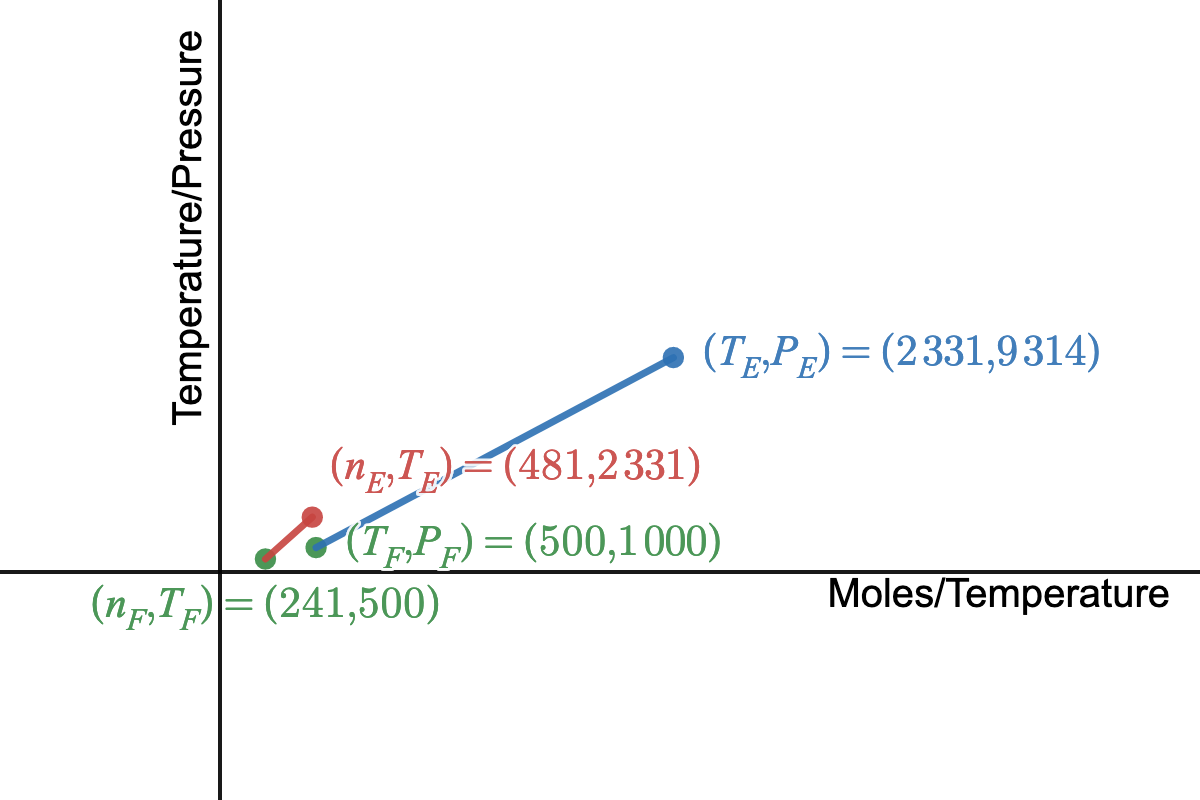
\includegraphics[width=.95\linewidth]{./images/desmos-example-1-1.png}
        \end{subfigure}
        \begin{subfigure}{0.49\linewidth}
            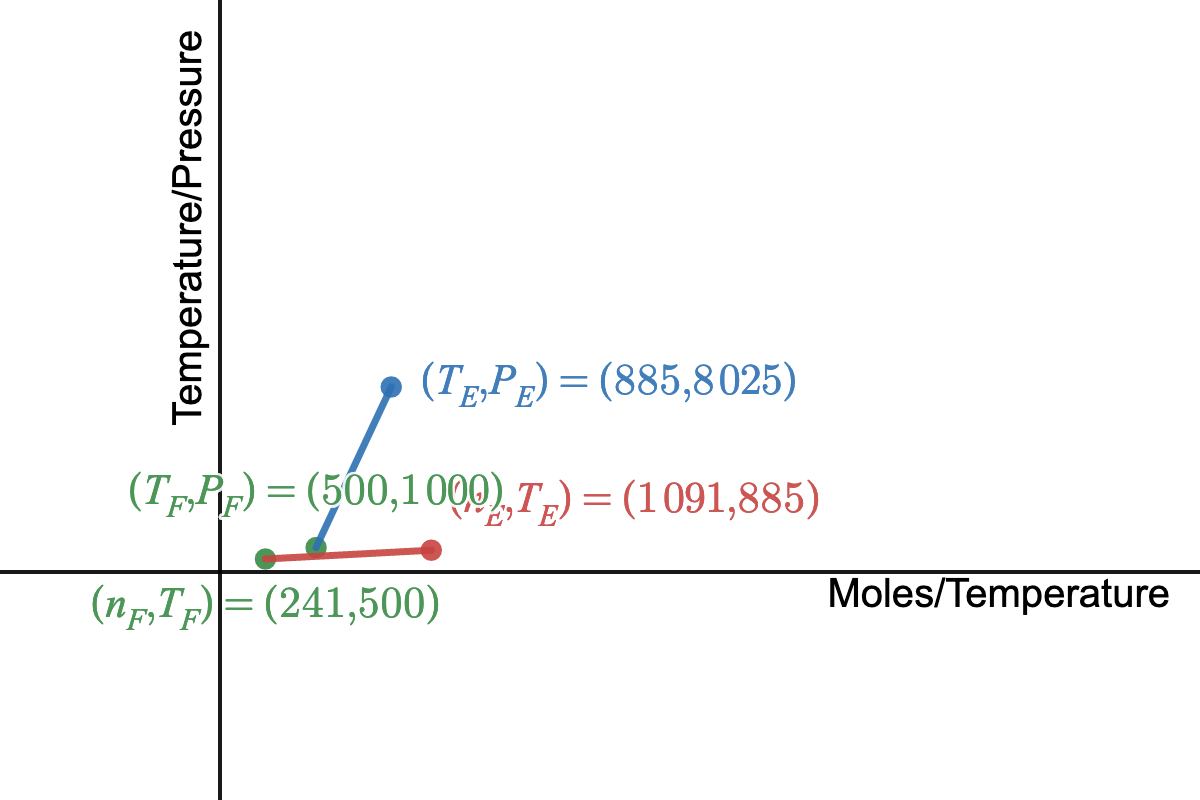
\includegraphics[width=.95\linewidth]{./images/desmos-example-1-2.png}
        \end{subfigure}
    \end{center}
    \caption{Desmos visualization of the affect of $n_R$, $n_H$ and $n_C$
    on the final temperature $T_E$ and pressure $P_E$.}
    \label{fig:desmos-1}
\end{figure}
\begin{example*}
    Suppose we have initial conditions $T_F=500$, $P_F=1000$, $T_C=200$ and $T_H=2500$,
    but we don't have a particular target pressure $P_T$ or temperature $T_T$;
    we just want to see how things change as we remove some amount $n_R$ from $F$,
    add some amount $n_H$ from $H$ into $F$,
    and/or add some amount $n_C$ from $C$ into $F$.

    Lets call $T_E$, $P_E$ and $n_E$ our end results: the temperature, pressure and number
    of moles after having removed $n_R$ and having added $n_I$.
    Our procedure is this: pick values for $n_R$, $n_H$ and $n_C$,
    \begin{enumerate*}[label=(\alph*)]
        \item calculate $n_E=(n_F-n_R)+n_I$ where $n_I=n_H+n_C$,
        \item calculate $T_E$ by solving $T_E n_E=T_F(n_F-n_R)+T_I n_I$
            (\cref{eq:T-combine}) for $T_E$, and then
        \item calculate $P_E$ by solving \cref{eq:ideal} for $P_E$.
    \end{enumerate*}

    First we need to calculate $n_F$, the initial amount of moles in the furnace, using
    \cref{eq:ideal} (recall that $V_F=1000$ and $R=8.314$):
    \[
        n_F
        = \frac{P_F\cdot V_F}{R\cdot T_F}
        = \frac{1000\cdot 1000}{8.314\cdot 500}
        \doteq 240.56 \text{ moles $\CDiox$}.
    \]
    (Alternatively, since this is Stationeers we're talking about, we would have been able to
    find this value just by reading the number of moles from the furnace:
    \mintinline{text}{l nF furnace TotalMoles}.)
    \begin{example*}[$n_R=100$, $n_H=200$ and $n_C=0$]
        \phantom{ }
        \begin{enumerate}[label=(\alph*)]
            \item
                \begin{math}
                    n_E=(240.56-100)+(200+0)=340.56
                \end{math}
            \item
                \begin{math}
                    \begin{aligned}[t]
                        T_E
                        &= (T_F(n_F-n_R)+(T_H n_H+T_C n_C))/n_E \\
                        &= (500\cdot 140.56+(2500\cdot 200+200\cdot 0))/340.56
                        \doteq 1674.54\text{ K}.
                    \end{aligned}
                \end{math}
            \item
                \begin{math}
                    \begin{aligned}[t]
                        P_E
                        &= (n_E\cdot R\cdot T_E)/V_F \\
                        &= (340.56\cdot 8.314\cdot 1674.54)/1000
                        \doteq 4741.32\text{ kPa}.
                    \end{aligned}
                \end{math}
        \end{enumerate}
    \end{example*}
    \begin{example*}[$n_R=0$, $n_H=0$, and $n_C=300$]
        \phantom{ }
        \begin{enumerate}[label=(\alph*)]
            \item
                \begin{math}
                    n_E=(240.56-0)+(0+300)=540.56
                \end{math}
            \item
                \begin{math}
                    T_E
                    % = (T_F(n_F-n_R)+(T_H n_H+T_C n_C))/n_E
                    = (500\cdot 240.56+(2500\cdot 0+200\cdot 300))/540.56
                    \doteq 333.51\text{ K}.
                \end{math}
            \item
                \begin{math}
                    P_E
                    % = (n_E\cdot R\cdot T_E)/V_F
                    = (540.56\cdot 8.314\cdot 333.51)/1000
                    \doteq 1498.84\text{ kPa}.
                \end{math}
        \end{enumerate}
    \end{example*}
    From these examples (and playing around on Desmos) we can see that it should be possible to
    construct a decent variety of target pressures and temperatures.

    Check out this quick
    \href{https://www.desmos.com/calculator/clfts6kzwk}{graph in Desmos} to help visualize
    what's going on (or see \cref{fig:desmos-1}).
\end{example*}


\subsection{Calculating minimal amounts}

We have enough bounds here to establish a system of equations with which we can solve the problem;
that is to be able to solve for a minimal amounts $n_R$ to remove, $n_H$ of $H$ to add and $n_C$ of
$C$ to add. It will be a matter of solving these equations for particular variables, and applying
certain metrics to solve for these minimal values.
Recall that what we want is for our furnace to end up at some target temperature $T_T$ and pressure
$P_T$. We will find there there's a whole lot of potential solutions in terms of $n_R$, $n_H$ and
$n_C$ (technically an infinite amount, even within the bounds we establish), but we can simplify
these solutions by selecting the ones which either minimize the amount removed from the initial
furnace volume, minimize the amount added from only $H$, or minimize the amount added from only $C$.

First, solve \cref{eq:T-combine-model-1} for $n_I$. This yields $n_I$ as a function of $n_R$ and
$T_I$; the remaining variables ($T_T$, $n_T$, $T_F$ and $n_F$) are all fixed:
\begin{equation}
    f(n_R,T_I) = n_I = \frac{T_T n_T-T_F(n_F-n_R)}{T_I}.
    \label{eq:f}
\end{equation}
\begin{figure}
    \begin{center}
        \begin{subfigure}{0.48\textwidth}
            \Surf[.7]{4000}{500}{9000}{700}{200}{2500}
        \end{subfigure}
        \begin{subfigure}{0.48\textwidth}
            \Surf[.7]{6000}{600}{5000}{800}{200}{2500} % red example
        \end{subfigure}
        \begin{subfigure}{0.48\textwidth}
            \Surf[.7]{15000}{900}{6000}{600}{200}{2500} % blue example
        \end{subfigure}
        \caption{The surface defined by $(n_R,T_I,f)$ for various initial conditions.}
        \label{fig:surf}
    \end{center}
\end{figure}
We can plot this function $f$, being of two variables $n_R$ and $T_I$, in three dimensions using the
bounds on $T_I$ and $n_R$: that $T_C\le T_I\le T_H$ and $0\le n_R\le n_F$. \cref{fig:surf}
visualizes this bounded surface for a few different initial conditions (and in these examples I
chose $T_C=200$ and $T_H=2500$).
\begin{note*}
    This surface we define by $(n_R,T_I,f)$ is in-fact a two-dimensional surface, although it is
    \emph{embedded} within three-dimensional space! That is, imagine that you are a point on this
    surface, and that you are not allowed to leave it. You can walk across this surface, but you
    cannot jump up off of it, and you cannot get below it, but you can still see above and below:
    you still stand within three-dimensional space but you cannot leave this two dimensional
    surface. This is what we mean by point solutions to equation \cref{eq:f}: a point in three
    dimensional space $(x,y,z)=(n_R,T_I,n_I)$ sits upon this surface if and only if
    $z=f(x,y)\Rightarrow n_I=f(n_R,T_I)$ is satisfied (that is, if after evaluating $f$ at $n_R$ and
    $T_I$, the equality $n_I=f(n_R,T_I)$ is indeed \emph{true}).
\end{note*}
Second, consider solving $n_T=(n_F-n_R)+n_I$ for $n_I$. We get $n_I=n_T-n_F+n_R$. This expresses
$n_I$ as a function of merely $n_R$, since both $n_F$ and $n_T$ are fixed:
\begin{equation}
    g(n_R) = n_I = n_T-n_F+n_R.
    \label{eq:g}
\end{equation}
Then lets take $f$ (\cref{eq:f}) and, instead of solving for $n_I$, solve for $T_I$:
\[
    n_I = \frac{T_T n_T+T_F(n_F-n_R)}{T_I}
    \Rightarrow
    T_I = \frac{T_T n_T+T_F(n_F-n_R)}{n_I}
\]
With this we keep $n_R$ as a free-variable, but replace $n_I$ with $g$ (\cref{eq:g}).
We'll call this newly constructed equation, of \emph{only one variable}, $h$:
\begin{equation}
    h(n_R) = T_I
    = \frac{T_T n_T+T_F(n_F-n_R)}{n_I}
    = \frac{T_T n_T+T_F(n_F-n_R)}{g(n_R)}.
    \label{eq:h}
\end{equation}
Consider the surface we previously defined by $(n_R,T_I,f)$ (\cref{fig:surf}).
We have to pick both $n_R$ and $T_I$ together, a \emph{pair} of points, from a mesh of points (the
Cartesian product of the $n_R$ and $T_I$ domains). However, now we have an expression $h(n_R)=T_I$
that is dependent on only this only variable $n_R$.
What we have then is that we can solve for $T_I$ in terms of of $n_R$
(\cref{eq:h}, $T_I=h(n_R)$), and then can solve for $n_I$ in terms of $n_R$ and $T_I=h(n_R)$
(\cref{eq:f}, $n_I=f\big(n_R,g(n_R)\big)$).

Effectively, we've reduced our previously two dimensional surface down to a one dimensional
\emph{curve} (a curve which is embedded within the surface, with the surface embedded within
three dimensional space).
\begin{figure}
    \begin{center}
        \begin{subfigure}{0.48\textwidth}
            \Curve[.6]{4000}{500}{9000}{700}{200}{2500}
        \end{subfigure}
        \begin{subfigure}{0.48\textwidth}
            \Curve[.6]{6000}{600}{5000}{800}{200}{2500} % red example
        \end{subfigure}
        \begin{subfigure}{0.48\textwidth}
            \Curve[.6]{15000}{900}{6000}{600}{200}{2500} % blue example
        \end{subfigure}
        \caption{
            The curve in red defined by $(n_R,g,f)$ embedded within the surface defined by
            $(n_R,T_I,f)$ (for the same various initial conditions).
        }
        \label{fig:curve}
    \end{center}
\end{figure}
And again we can plot this; see \cref{fig:curve} in which we can see the curve embedded within
the surface.

So we now have values for both $T_I$ and $n_I$ in terms of whatever we pick for $n_R$.
However $n_I$ is not just some amorphous gas mixture, but a particular combination of moles from
$C$ and moles from $H$---which we can now solve for.
Consider the equations
$n_I=n_H+n_C$ (\cref{eq:n-combine-model-1}) and
$T_I n_I=T_H n_H+T_C n_C$ (\cref{eq:T-combine-model-1});
solve the first in terms of $n_C$:
\[
    n_I=n_H+n_C \Rightarrow n_C=n_I-n_H
\]
For the second, recognize that $T_I$, $n_I$, $T_H$ and $T_C$ are all fixed; all except for $n_H$ and
$n_C$. But we solved the first equation for $n_C$. Thus, substitute $n_C$ with $n_I-n_H$ in the
second equation and solve for $n_H$:
\begin{equation}
    T_I n_I
    = T_C n_C+T_H n_H
    = T_C(n_I-n_H)+T_H n_H
    \Rightarrow
    n_H = \frac{n_I(T_C-T_I)}{T_C-T_H}.
\end{equation}
So that now we have $n_H$ as a function of everything we previously calculated, and $n_C$ is simply
$n_I-n_H$,
\begin{itshape}
    and to an extent we have completely solved the proposed problem! Given our initial conditions
    and chosen target pressure and temperature, we can now choose any $n_R$ in the range $0$ to
    $n_F$ with which we can calculate exactly the number of moles $n_C$ from $C$ and $n_H$ from $H$
    to combine into $I$ so that when we add $I$ into $F$ we precisely hit our target temperature and
    pressure.
\end{itshape}

\emph{That being said, we're not quite done\ldots}
\begin{example*}
    Lets consider the third example of \cref{fig:curve}, where our initial conditions are
    $P_F=15000$ and $T_F=900$, and target conditions are $P_T=6000$ and $T_T=600$.

    Using Desmos again, I've sketched up
    \href{https://www.desmos.com/calculator/h7vtybqa5r}{the model so far}
    (\cref{fig:desmos-2})
    and plugged in these initial conditions.
    By moving the $n_R$ slider, notice that calculated values $T_E$ and $P_E$ (our final temperature
    and pressure) are exactly $T_T$ and $P_T$ (our targets), always.

    However, try lowering the value of $n_R$ and observe the values of $n_H$ and $n_C$;
    one or both of them go negative! These values are \emph{mathematically correct}, but intuitively
    it makes no sense to add a \emph{negative} amount of $C$ or $H$\ldots
\end{example*}
As the example above demonstrates, we're not actually done. We've solved for all
real-solutions to the problem, but we've neglected the bound that we cannot add a negative amount of
$C$ or $H$. Looking back at the third example of \cref{fig:curve}, notice that the curve exits
to the right of the graph. This shows us that not all values of $n_R$ are valid for our model,
because for some values (where the curve leaves the graph) we are adding a negative amount of $C$ or
$H$.
\begin{figure}
    \begin{center}
        \begin{subfigure}{0.49\linewidth}
            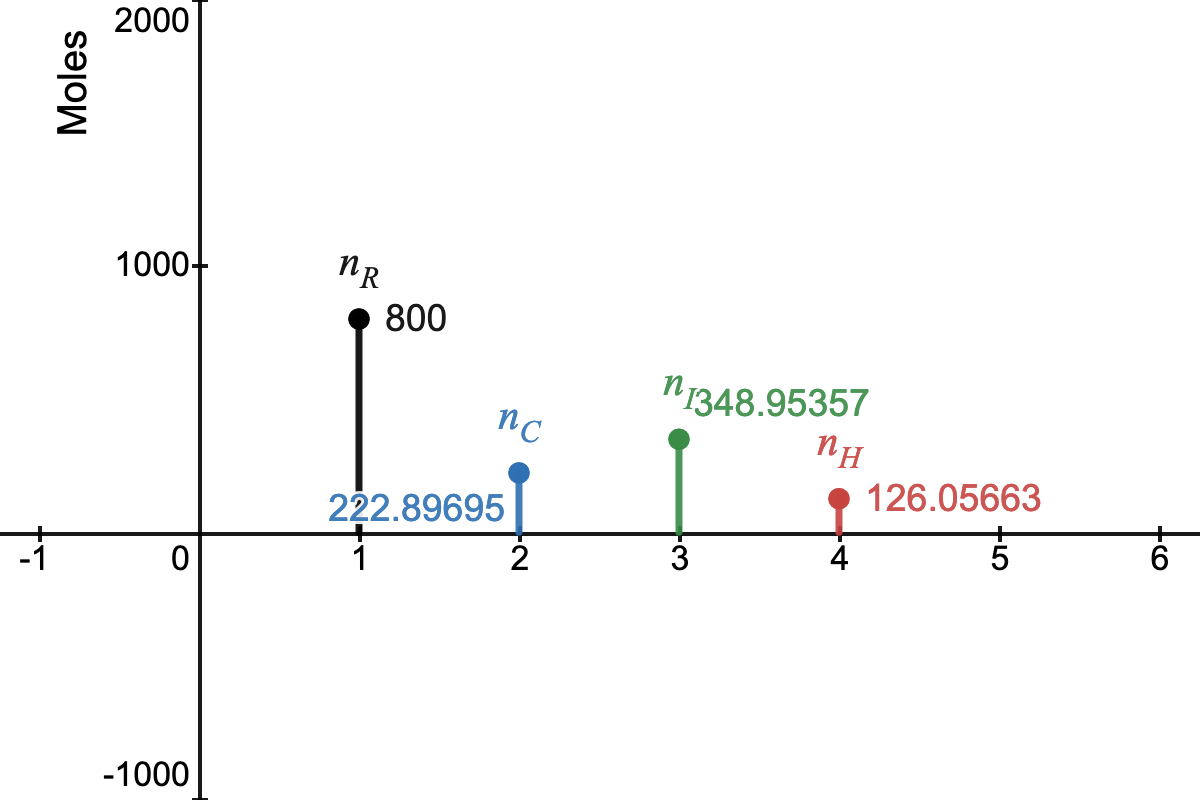
\includegraphics[width=.95\linewidth]{./images/desmos-example-2-1.png}
        \end{subfigure}
        \begin{subfigure}{0.49\linewidth}
            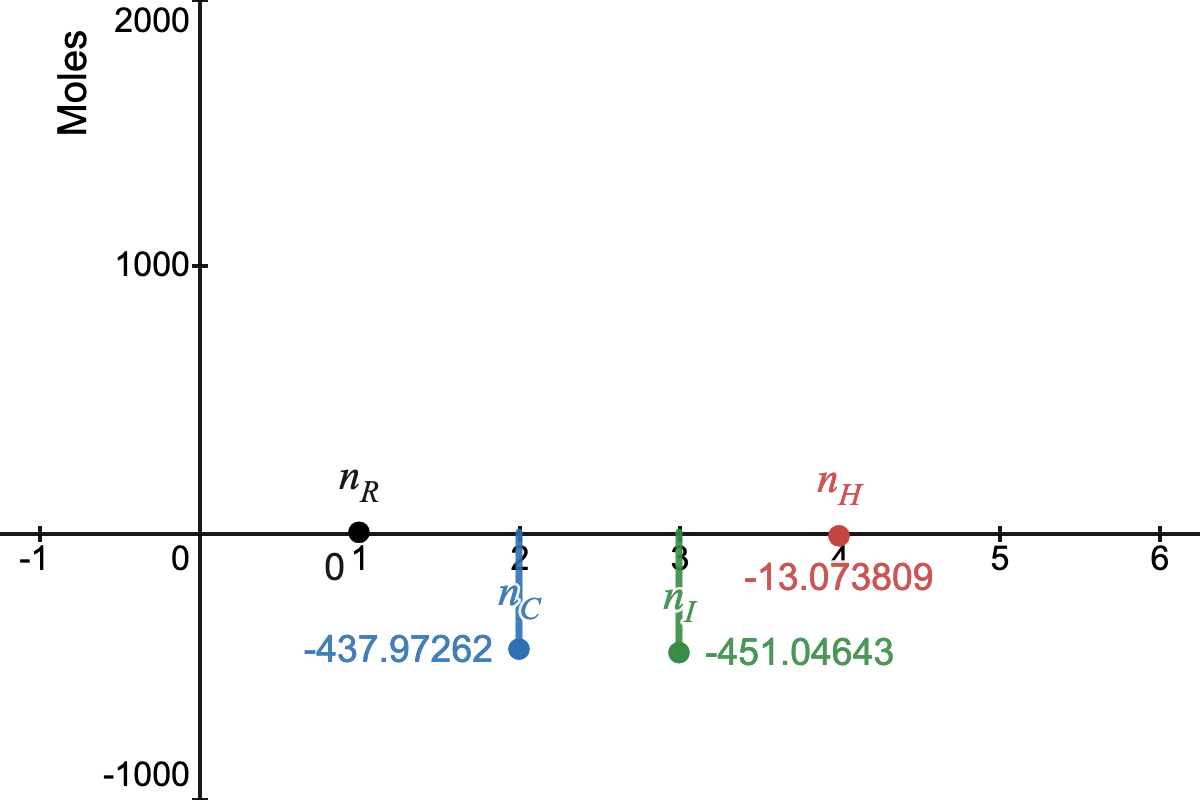
\includegraphics[width=.95\linewidth]{./images/desmos-example-2-2.png}
        \end{subfigure}
    \end{center}
    \caption{Desmos visualization of the $n_R$, $n_I$, $n_H$ and $n_C$ relationships.}
    \label{fig:desmos-2}
\end{figure}

To address this, consider the energy quantity $T_I n_I$. So far we have not bounded this quantity,
but in fact $T_I$ is bounded by $T_C\le T_I\le T_H$. We can use these inequalities to solve for
a true lower bound to $n_R$ by substituting $n_I=n_T-n_F+n_R$ (\cref{eq:n-combine-model-1})
and $T_I n_I=T_T n_T-T_F(n_F-n_R)$ (from solving \cref{eq:T-combine-model-2} for $T_I n_I$).
% \begin{paracol}{2}
%     \switchcolumn
% \end{paracol}

First solving for $n_R$ via $T_C n_I\le T_I n_I$:
\begin{alignat*}{2}
    &\phantom{\Rightarrow\ }&
    T_C n_I &\le T_I n_I \\
    &{\Rightarrow\ }&
    T_C(n_T-n_F+n_R) &\le T_T n_T - T_F(n_F-n_R) \\
    &{\Rightarrow\ }&
    T_C n_T - T_C n_F + T_C n_R &\le T_T n_T - T_F n_F + T_F n_R \\
    &{\Rightarrow\ }&
    T_C n_T - T_T n_T + T_F n_F - T_C n_F &\le T_F n_R - T_C n_R \\
    &{\Rightarrow\ }&
    n_T(T_C - T_T) + n_F(T_F - T_C) &\le n_R(T_F - T_C)
\end{alignat*}
\begin{equation}
    \Rightarrow n_{R_H} = \frac{n_T(T_C - T_T)}{T_F - T_C} + n_F \le n_R.
    \label{eq:C-bound}
\end{equation}
And second, solving for $n_R$ via $T_I n_I\le T_H n_I$:
\begin{alignat*}{2}
    &\phantom{\Rightarrow\ }&
    T_I n_I &\le T_H n_I \\
    &{\Rightarrow\ }&
    T_T n_T - T_F(n_F-n_R) &\le T_H(n_T-n_F+n_R) \\
    &{\Rightarrow\ }&
    T_T n_T - T_F n_F + T_H n_F &\le T_H n_T - T_H n_F + T_H n_R \\
    &{\Rightarrow\ }&
    T_T n_T - T_H n_T + T_H n_F - T_F n_F &\le T_H n_R - T_F n_R \\
    &{\Rightarrow\ }&
    n_T(T_T - T_H) + n_F(T_H - T_F) &\le n_R(T_H - T_F)
\end{alignat*}
\begin{equation}
    \Rightarrow n_{R_C} = \frac{n_T(T_T - T_H)}{T_H - T_F} + n_F \le n_R.
    \label{eq:H-bound}
\end{equation}
The names $n_{R_H}$ and $n_{R_C}$ that I have chosen might be confusing and appear to be backwards,
but this is what these two lower bounds are actually telling us about $n_R$:
\begin{itemize}
    \item The lower bound $n_{R_C}$, despite being a function of $T_H$,
        tells us that if we remove an amount less than $n_{R_C}$ (i.e. if $n_R<n_{R_C}$),
        then $n_C$ becomes negative; and\ldots
    \item The lower bound $n_{R_H}$, despite being a function of $T_C$,
        tells us that if we remove an amount less than $n_{R_H}$ (i.e. if $n_R<n_{R_H}$),
        then $n_H$ becomes negative.
\end{itemize}
So since we know that we are not allowed to remove an amount less than either of these bounds, nor
are we allow to remove less-than zero, we can simplify the bounds on $n_R$ once-and-for-all:
\begin{equation}
    n_{R_{\min}} \le n_R \le n_F, \quad
    \text{where } n_{R_{\min}} = \max(0,n_{R_C},n_{R_H}).
    \label{eq:n_R-bound}
\end{equation}
So we have fixed the range for $n_R$ but we haven't actually said what value to choose.
Now, there's some analysis we could apply to help study this curve (and that might be something I
relearn later to include here), but from the visualization we can also clearly see that where this
curve will always intersect the boundaries of the graph \cref{fig:full} is actually the point at
which not only $n_R$ is minimal, but so is $n_C$ and $n_H$ (by virtue of minimizing $n_I$).

\begin{itshape}
    Therefore, $n_{R_{\min}}$ doesn't just give us the range for $n_R$ but it actually gives us the
    minimal point!
\end{itshape}
\begin{figure}
    \begin{center}
        \begin{subfigure}{0.48\textwidth}
            \Full[.6]{4000}{500}{9000}{700}{200}{2500}
        \end{subfigure}
        \begin{subfigure}{0.48\textwidth}
            \Full[.6]{6000}{600}{5000}{800}{200}{2500} % red example
        \end{subfigure}
        \begin{subfigure}{0.48\textwidth}
            \Full[.6]{15000}{900}{6000}{600}{200}{2500} % blue example
        \end{subfigure}
        \caption{
            The surface $(n_R,T_I,f)$, the curve $(n_R,g,f)$, and a point $(n_R,g,f)$ where
            $n_R$ is determined to be $\max(0,n_{R_C},n_{R_H})$.
        }
        \label{fig:full}
    \end{center}
\end{figure}

We have, in the end, a final theorem to use in the application of solving the problem within
Stationeers:
\begin{thm}[Acquiring $T_T$ and $P_T$ with minimal $n_R$, $n_C$ and $n_H$]

    Fix a single gas furnace system $F$ with initial temperature $T_F$ and pressure $P_F$, a target
    temperature $T_T$ and target pressure $P_T$, a cold source $C$ with temperature $T_C\le T_T$,
    and a hot source $H$ with temperature $T_H\ge T_T$.

    The point $(n_R,n_C,n_H)$ which satisfies $T_T n_T=T_F(n_F-n_R)+T_I n_I$ that minimizes the
    values of $n_R$, $n_H$ and $n_C$ is given by the following algorithm:
    \begin{multicols}{2}
        \begin{enumerate}[label=(\alph*)]
            \item $n_T = \dfrac{P_T V_F}{R T_T}$,
            \item $n_{R_C} = \dfrac{n_T(T_T - T_H)}{T_H - T_F} + n_F$,
            \item $n_{R_H} = \dfrac{n_T(T_C - T_T)}{T_F - T_C} + n_F$,
            \item ${\color{colorA}n_R} = n_{R_{\min}} = \max(0, n_{R_C}, n_{R_H})$,
            \item $n_I = n_T - n_F + n_R$,
            \item $T_I = \dfrac{T_T n_T - T_F(n_F - n_R)}{n_I}$,
            \item ${\color{colorA}n_H} = \dfrac{n_I(T_C - T_I)}{T_C - T_H}$,
            \item ${\color{colorA}n_C} = n_I - n_H$.
        \end{enumerate}
    \end{multicols}
\end{thm}

% \begin{example*}
%     Again considering the initial conditions of \cref{fig:curve}'s third case
%     ($P_F=15000$, $T_F=900$, $P_T=6000$, $T_T=600$) we can now calculate a correct lower bound:
%     \[
%         n_{R_C} \doteq 75.17, \quad
%         n_{R_H} \doteq 530.18, \quad
%         n_{R_{\min}} = \max(0,n_{R_C},n_{R_H}) = 530.18.
%     \]
% \end{example*}

% ; thus $n_{R_C}$ is the true lower bound.
% So to account for these impossibilities, we


% \cref{eq:C-combine}
% \cref{eq:T-combine}

% Our goal: 
\end{document}
